\section{\sysname}
\label{sec:system}
% Basic what it is
\sysname is a slim, batteryless, occupancy monitoring sensor system mounted to the top of a doorframe.
It is powered by energy harvested from two arrays of indoor solar panels pointed at the floor.
The panels serve two roles: 1)~energy harvester and 2)~sensor.
These panels gather \textbf{energy} for computation, sensing, and signaling while also providing the \textbf{signal} that \sysname uses to detect when a person walks through the doorway, in the form of variations in the harvested energy.
\sysname records the direction---entry or exit---of each doorway event and stores this information in non-volatile memory for later transmission.


\noindpar{Design Goals:} Unpredictable power availability coupled with confounding factors of human based sensing make designing an intermittently powered occupancy sensor challenging.
We designed \sysname to meet the following design goals which address specific challenges:
\begin{enumerate}
	\item \textbf{Availability:} Doorway events can occur at any time.
	While many intermittent sensors are able to gather data opportunistically as energy is available, \sysname is designed to conserve its harvested energy, so that it is available to detect ephemeral doorway events, whenever they occur.
	\item \textbf{Accurate direction:} In addition to detecting someone passing through the doorway, \sysname uses angled solar panels to accurately determine their direction.
	This plays a crucial role in inferring the occupancy of rooms and buildings.
	\item \textbf{Variable lighting conditions:} Indoor lighting conditions can change over time, due to human behavior and the relative movement of the sun.
	We have designed \sysname to work in a range of different lighting conditions by using detection circuits that respond to changes in light level, independent of the absolute amount of light, as well as tuning mechanisms built into the prototype.
	\item \textbf{Variable human characteristics:} An effective occupancy sensor should work well in spite of variations in clothing, hair, height, walking speed, and skin color. By focusing on changes in total reflected light, \sysname is robust to these human variations.
	\item \textbf{Form factor:} We want \sysname to be easy to deploy, to fit unobtrusively inside a door frame, and avoid contact with doors (on frames with doors).
	We could harvest more energy by wrapping \sysname around the doorframe, but the system would be more expensive, harder to deploy, and more likely to interfere with doors, while changing the aesthetics of the doorway.
\end{enumerate}

\noindpar{What \sysname is not.}
We also want to be clear about what \sysname is \emph{not}.
\sysname is \emph{not} a security device.
\sysname helps building owners and managers understand how people move through buildings, but it is \emph{not} designed to thwart malicious behavior.
We can easily trick \sysname with a flashlight or reflective materials, and we can disable it completely by covering its solar panels or turning off the lights.
Users looking to prevent shenanigans or tomfoolery should use a different device.
Users looking for a long-lived, low-maintenance, best-effort batteryless occupancy sensor for monitoring normal behaviors should read on.

% fig refs
An overview of the \sysname architecture is shown in \figref{fig:overview} and our \sysname prototype device is shown in \figref{fig:prototype}.
% Intro the rest of the section
We detail our approach to meeting these design goals and answering their associated challenges in the rest of the section~--- specifically we describe the \sysname architecture and design, the detection mechanism, and the energy management operations.


\begin{figure}[t]
\centering
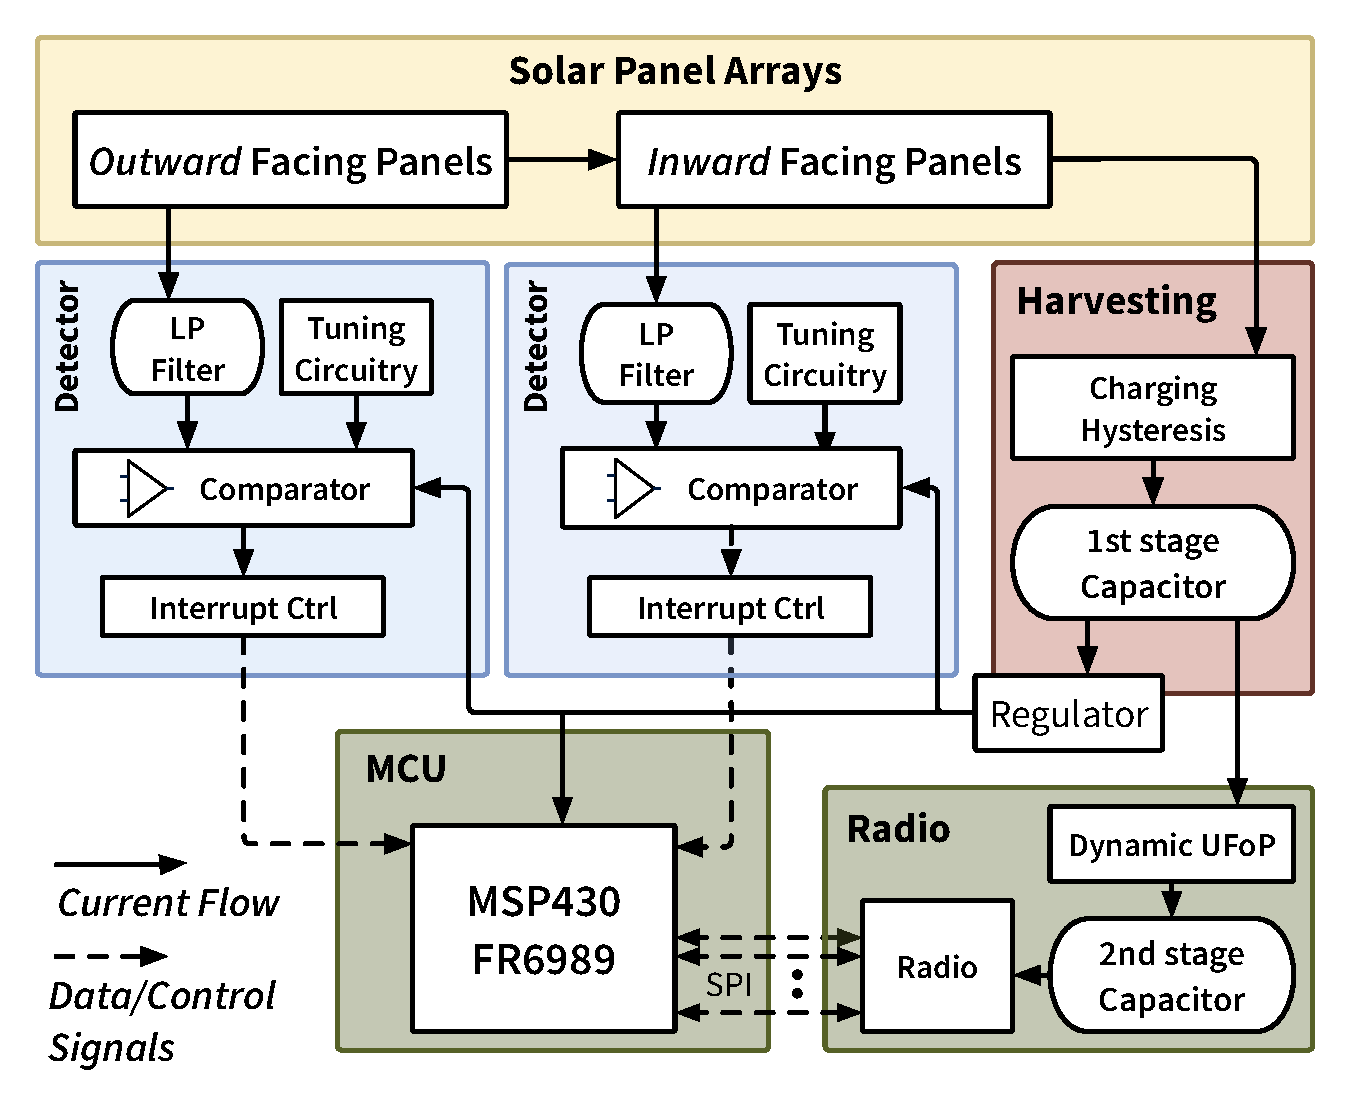
\includegraphics[width=\columnwidth]{figs/overview.pdf}
\caption{The \sysname architecture overview. \sysname uses the energy and signal from two sets of solar panels to both power the sensor and detect people passing into and out of a doorway. Two detector circuits each monitor half of the solar panels mounted in series that face inward, and outward in the doorway. On detection, the detectors wake up the MCU to process, log, or communicate occupancy information.  \label{fig:overview}}
\end{figure}


\subsection{Energy Harvesting and Management}
\sysname takes advantage of the ubiquity of indoor light in homes and offices.
Solar panels are mounted to the top of the door frame, pointing down toward the floor---half tilted \ang{20} inward and half tilted \ang{20} outward.
Pointing the panels downward is not ideal for energy harvesting but effective for detecting doorway events and provides a slim, easy-to-deploy form factor.
The \ang{20} tilt helps \sysname determine walking direction, as a person will affect one half of the panels before the other.

To maximize energy harvesting, we connect the two sets of solar panels---the inward-facing set and the outward-facing set---in series.
A series configuration conveniently combines the two panel sets into a single power source, but we can't directly measure the raw voltage on each set since the sets lack a common reference ground\footnote{For a series connection, we connect the positive terminal of the first panel set to the negative terminal of the second.}.
Instead, we measure the voltage of the outward-facing set alone, and the combination of the two sets.
We could compute the inward panels' voltage by subtracting the two; however, we have found that we can skip this step and just compare the two measurements directly, as shown in \figref{fig:traces}, to determine walking direction.

%Therefore, we feed the signal from one set of solar panels into one detector and the combination of the two sets into the other detector, which is sufficient to provide direction information.

\sysname uses federated energy storage~\cite{jhester:ufop:sensys} to power its microcontroller and peripherals.
Harvested solar energy is fed into a common first-stage storage capacitor and then automatically federated to its peripherals.
Federating energy allows us to prioritize detection and computation while saving up energy for more energy-expensive radio transmissions.
It also improves harvesting efficiency and allows separation of peripherals without fear that the microcontroller will lose power due to a radio transmission.
\sysname currently supports connections for two peripherals --- a Texas Instruments CC1101 radio and an extra slot for potential expansion to be used in future work.
%We plan to add additional sensors to our design in the near future.
\begin{figure*}[t]
	\centering
	\begin{subfigure}[b]{0.5\textwidth}
		\centering
		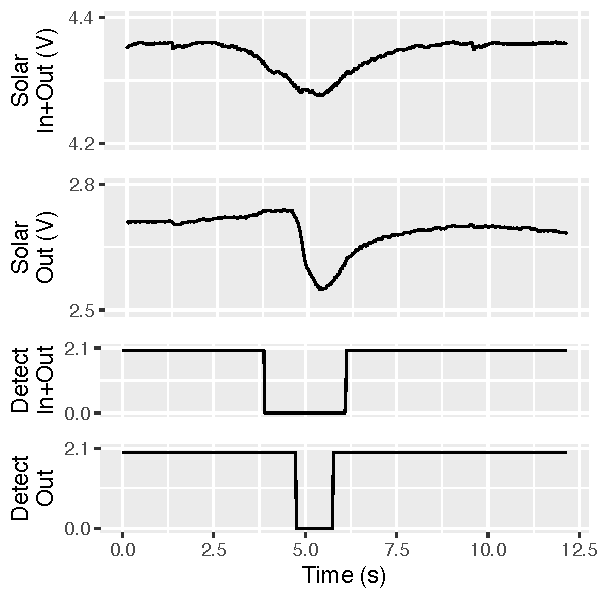
\includegraphics[width=\columnwidth]{figs/tracesin.pdf}
		\caption{Walking in.}
		\label{fig:tracesin}
	\end{subfigure}%
	%
	\begin{subfigure}[b]{0.5\textwidth}
		\centering
		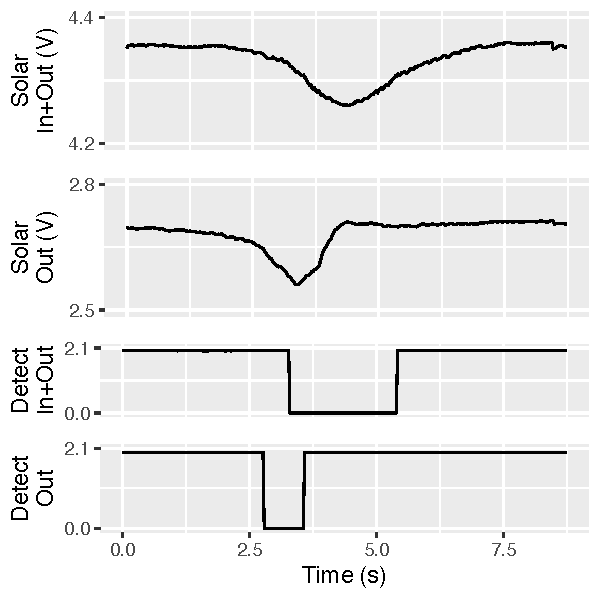
\includegraphics[width=\columnwidth]{figs/tracesout.pdf}
		\caption{Walking out.}
		\label{fig:tracesout}
	\end{subfigure}
	\caption{These traces show example solar panel voltages and detector outputs over time when a person walks through a \sysname-enabled doorway. The top traces show how the solar panel's voltages are deformed during the doorway event. The detector triggers are used to wake up the microcontroller and detect events and their direction. The angling of the panels cause the inward facing and outward facing detectors to trigger at different times depending on the direction the person is walking.\label{fig:traces}}
\end{figure*}

\subsection{Detection}
\label{sec:detection}



%\fxnote{[It would be nice to do this data driven off some traces gathered. Simulate, essentially, just by doing some light math. So how do we capture the waveforms when we trigger the wakeup? - JDH]}

%what happens when a person walks through.
When someone walks under \sysname, she blocks some of the reflected light hitting the solar panels.
In \figref{fig:traces}, the ``solar'' traces on top shows how the voltage from the solar panels changes during a doorway event.

In order to detect a doorway event, we could use an ADC to continuously measure the solar panel voltage over time and analyze those readings to detect the presence and more importantly, direction of motion.
Voltage levels and waveform shapes vary with lighting conditions, especially when one side of the doorway has more natural light, and this approach would require sophisticated signal analysis and prohibitive energy consumption.

Instead, \sysname uses a \textbf{detection circuit} that wakes up the microcontroller when it detects a significant change in the solar panel voltage over a short period of time.
This circuit consists of a passive first-order capacitive filter connected to a nano-power comparator---producing a square wave that transitions when the voltage increases or decreases faster than a set rate.
These transitions trigger interrupts that help \sysname detect when someone is passing through the doorway.

In order to determine movement direction, we use two detector circuits: one that detects change on the outward-facing panels and another that detects change on the combined inward- and outward-facing panels.
When someone walks through the doorway, the detectors trigger at different times, depending on the walking direction, as shown in \figref{fig:traces}.
\sysname compares the timing of these detector interrupts to distinguish incoming and outgoing doorway events.


\noindpar{Removing light flicker.}
Many fluorescent indoor lights flicker at \SI{60}{\hertz} or higher---a much higher frequency than the events \sysname is designed to detect.
These flucturations can confuse the detection circuit and produce false positives unless they are filtered out.
We add a low-pass filter to remove noise above \SI{10}{\hertz} from the solar panel signal.
%\figref{fig:flicker} shows the impact of the noise to the light signal both before and after filtering out the higher frequencies from the signal.

\noindpar{Isolating harvesting from sensing.}
If connected directly, \sysname's harvesting and event detection circuits conflict in two important ways.
First, the harvesting circuit stores harvested energy in a \SI{100}{\micro\farad} capacitor---a size that ensures that \sysname can store enough energy for short-term tasks and dampens the low-frequency voltage fluctuations that we need in order to detect doorway events.
Second, short-term power spikes from interrupt service routines and other computation cause high-frequency dips in the solar voltage, which can confuse the detection circuits.
We address both of these challenges by adding an additional low-pass filter between the detection and harvesting circuits, which isolates the solar panel from the load, and allows the solar panel voltage (after the initial flicker filter) to fluctuate over a wider range in response to doorway events with less interference from the storage capacitor, the microcontroller power draw, and the detector circuit power draw.


\noindpar{Detection algorithm:}
During normal operation, when \sysname is not in a doorway event, the MCU remains in deep sleep.
While in deep sleep, the MCU is only triggered awake by the detector circuits going from high to low---designating the beginning of a doorway event, from the change in solar harvesting energy from the light occluded by a person walking through the doorway.
Once triggered, the MCU starts a timer (a few seconds), and records the time at which the interrupt occurred, then goes into sleep mode, waking up throughout the doorway event to capture the length of time between each detector's status change (from HIGH to LOW and vice versa).
Multiple interrupts often fire during a single doorway event as the person does not block light to the panels in an exact and smooth manner.
The timer defines the boundaries for what will be considered part of the event.

Times are recorded for the first falling edge interrupt and the last recorded rising edge for both solar panel groups.
When the timer fires, both solar panel groups' start and end times are compared to determine the direction of the event (entry or exit), and the \sysname stores the detected event in non-volatile memory.


In rare cases, only one detector detects the event.
These events are reported as a partial event, which doesn't have direction information.
Partial doorway events can occur when a person walks by the doorway but not through it (close enough to interfere with one panel group).


\subsection{Communication and Infrastructure}
The data that \sysname collects about people walking through is stored in non-volatile memory until it has enough energy to make a radio transmission.
The current setup collects data for a certain fixed number of events before it polls the radio to see if it is available.
If there is energy, then it will send statistics for the collected data, clearing its buffer.
If the capacitor for the radio isn't sufficiently charged, it will go back to sleep and try again after each subsequent event.
This way, we can keep collecting data as events occur, and transmit it all to the base station when we have sufficient power to do so.
%\fxnote{[Remove this - JDH]}

%\subsection{Adaptation}
%\fxnote{[Remove this - JDH]}

%\sysname dynamically changes task sets depending on energy availability - attempting to assign higher energy tasks when energy is more available in the environment and assigning lower energy tasks assigned when energy is scarce in the environment. \fxnote{[Does not do this, need to remove - JDH]}
%These tasks correspond to different tiers of quality of service (QoS) of the application, with the highest level providing real time event marking on door traffic coupled with person identification using heights, hair color, and wardrobe. \fxnote{[Does not do this either, need to remove - JDH]}
%The lowest QoS tier corresponds to only logging entry and exit, and sending a summary of the data opportunistically over the radio. \fxnote{[Does not do this either! Put in future work- JDH]}
